% Chapter Template

\chapter{Ensayos y resultados} % Main chapter title
\label{Chapter4} % Change X to a consecutive number; for referencing this chapter elsewhere, use \ref{ChapterX}

La idea de esta sección es explicar cómo se hicieron los ensayos, qué resultados se obtuvieron y analizarlos.

%----------------------------------------------------------------------------------------
%	SECTION 1
%----------------------------------------------------------------------------------------

\section{Diseño logrado}

Luego del primer diseño esquemático se fabrico un prototipo que puede verse en la figura  \ref{fig:proto1}. Debido a la inexperiencia en el uso del programa cad de diseño se realizo un mal manejo del grid de trabajo en el esquemático, por lo que las conexiones hechas en la hoja esquemática no aparecían en el PCB, esto llevo a que lineas que aparecían conectadas no lo estuvieran, por ende las conexiones de alimentación del integrado de medición eran erróneas, como también la de los dos transistores discretos.

\begin{figure}[!htb]
	\centering
	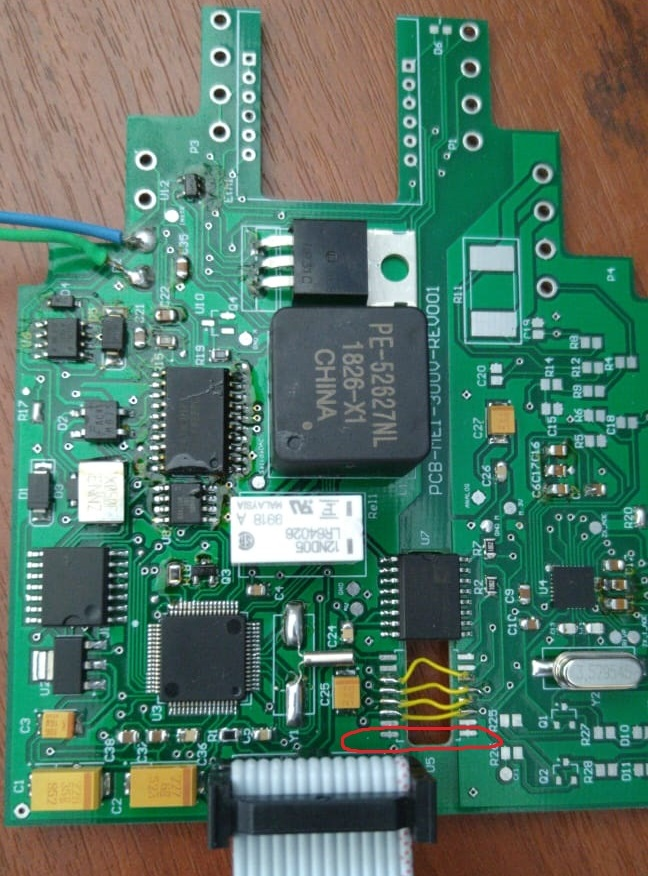
\includegraphics[width=80mm,keepaspectratio]{Figures/placaarmada1.jpeg}
	\caption{Primer PCB fabricado con conexiones arregladas.}
	\label{fig:proto1}
\end{figure}

Viendo las importantes faltantes en la placa, se procedió a corregir el diseño en el esquemático. Las conexiones faltantes se realizaron soldando cables en los terminales correspondientes, esto puede verse en la figura \ref{fig:parchess2}. Una vez asegurado el funcionamiento de los módulos se procedió a testear la placa.

\begin{figure}[!htb]
	\centering
	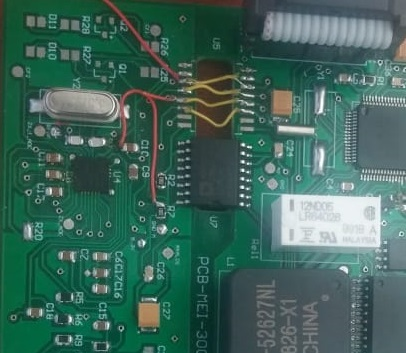
\includegraphics[width=60mm,keepaspectratio]{Figures/parche2.jpg}
	\caption{Soldado de cables para corregir el prototipo del PCB.}
	\label{fig:parchess2}
\end{figure}

\section{Pruebas sobre \textit{hardware}}
\label{sec:pruebasHW}

Se utilizo el primer prototipo para hacer las pruebas. Se realizaron mediciones sobre una lampara de 100 W para probar el funcionamiento del integrado de medición y las funcionalidades del software.

Se probo desconectar y conectar las tensiones de entrada para probar la reacción de la placa y corregir problemas que presentara en el software. Gracias a esto se detectaron errores en la comunicación 

Se utilizaron los puertos RS232 y RS485 para probar la comunicación por protocolo modbus.

\section{ Verificación de requerimientos}

Durante las pruebas se verificaron los requerimientos solicitados.

\subsection{Grupo de requerimientos referidos a alimentación eléctrica}
\begin{itemize}
\item El dispositivo deberá alimentarse con tensión continua. La tensión de alimentación deberá ser inferior a 30 V y superior a 12V.
\end{itemize}

Se probo que el prototipo logrado maneje tensiones de alimentación de 12 a 30 volts.

\subsection{Grupo de requerimientos referidos a medición de potencia del equipo}
\begin{itemize}
\item Capaz de realizar la medición de tensión alterna de una línea monofásica de baja tensión de Argentina, entrada de medición para 220V o 380V con una tolerancia de +/-15\%.
\end{itemize}

Se logro medir tensiones alternas de una linea monofásica de baja tension con tolerancia inferior al 15\%.

\begin{itemize}
\item Capaz de realizar la medición de corriente alterna de una línea monofásica de baja tensión de Argentina, hasta 5 A.
\end{itemize}

Se implemento una resistencia shunt de 4 mili ohms para realizar mediciones hasta 10 amperes. La intensidad de corriente eléctrica que tolera el shunt es alrededor de 30 amperes.

\begin{itemize}
\item Capaz de realizar la medición de potencia eléctrica activa de una línea monofásica de baja tensión de Argentina, hasta 4000 W.
\end{itemize}

Se implemento un arreglo de resistores para lograr medir efectivamente hasta 495 volts. Por lo que se puede llegar a medir hasta la potencia solicitada.

\begin{itemize}
\item El sistema de medición que se utilizará para las mediciones deberá ser aislado de la salida de comunicaciones del puerto serie.
\end{itemize}

Todos las circuitos de medición se encuentran aislados de los puertos de comunicación serie por lo que se considera resuelto este requisito.

\subsection{Grupo de requerimientos referidos a Interfaces de comunicación}
\begin{itemize}
\item Deberá realizar las comunicaciones a través de protocolos RS485 y RS232.
\end{itemize}

Se establecieron dos salidas diferentes de la placa por las cuales cada una funciona por un estándar diferente. Se adaptaron los niveles de tension para que cada salida fuera capaz de manejar los protocolos deseados.

\begin{itemize}
\item Deberá contemplar una posible modificación a futuro para una interfaz ethernet a través de una entrada para rj45.
\end{itemize}

Se dejo en el PCB el grabado del footprint de un modulo wiz820io con puerto ethernet y se realizaron los cortes necesarios para que quepa en la carcasa para riel DIN.
 

\subsection{Grupo de requerimientos referidos a diseño del circuito eléctrico}
\begin{itemize}
\item El dispositivo deberá poseer como microcontrolador principal MSP430F2418
\end{itemize}

Se uso el microcontrolador MSP430F2418 de \textit{texas instrument} con una referencia de tensión externa y un cristal oscilador de 32768 Hz.

\begin{itemize}
\item Se implementaran protecciones contra sobretensión en salida y entradas
\end{itemize}

La entrada de alimentación, y la salida de enlace de corriente tienen protección de sobretensión. 

\begin{itemize}
\item Deberá poseer un relé para realizar un corte por corriente.
\end{itemize}

Se conecto al microcontrolador un relé para accionarlo según las necesidades.

 
\subsection{Grupo de requerimientos referidos a diseño  de impresión del circuito}
\begin{itemize}
\item Se contempla en el diseño que el tipo de soldado será por refusión por cara superior.

\item Se contempla en el diseño que el tipo de soldado será por ola en la cara inferior del circuito.
\end{itemize}

Ambos requerimientos se cumplieron en la elaboración del prototipo.

\section{Realización de un manual de usuario}

Al finalizar las correcciones sobre el software se elaboro un manual de usuario en un documento online publico donde se especifica el uso del dispositivo armado, sus partes y conexiones, especificaciones de que parámetros puede medir y los registros que comunica por protocolo modbus.


\begin{figure}[!htb]
	\centering
	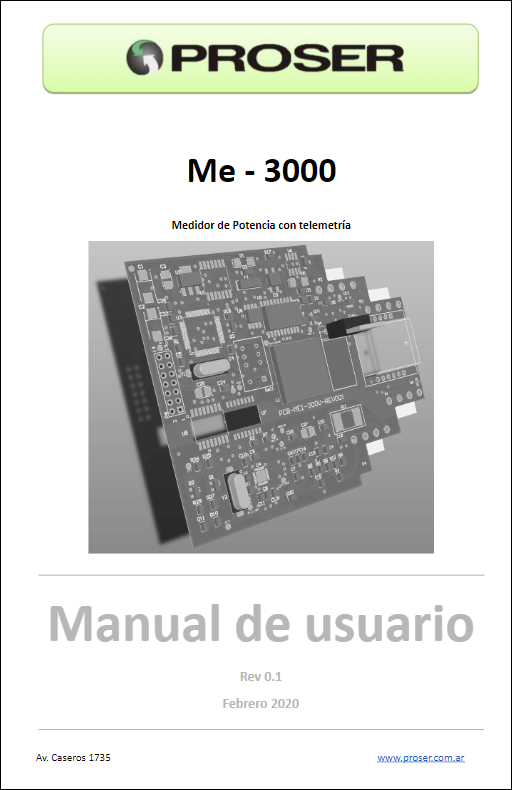
\includegraphics[width=80mm,keepaspectratio]{Figures/portadamanual.png}
	\caption{Portada del manual elaborado.}
	\label{fig:proto1}
\end{figure}

